

\subsection{Training}




\subsection{Evaluating}

\begin{figure}[H]
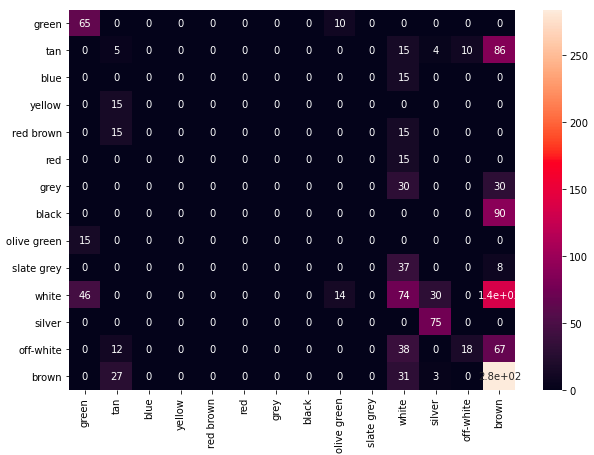
\includegraphics[scale=0.45]{latex/images/Heatmapbefore.png}
\label{fig:Heatmapbefore}
\caption{Predictions of color questions before training with new questions}
\end{figure}

\begin{figure}[H]
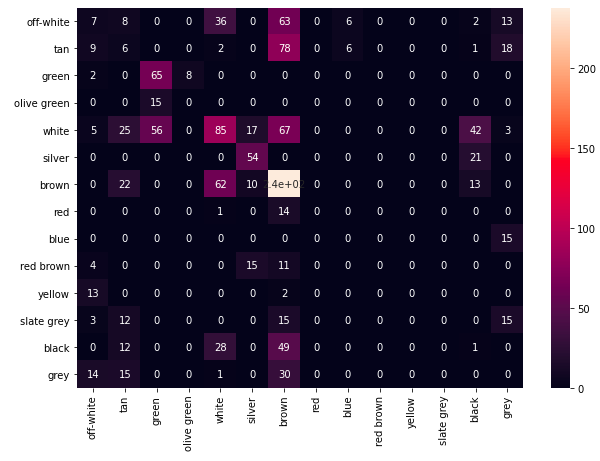
\includegraphics[scale=0.45]{latex/images/HeatmapAfter.png}
\label{fig:HeatmapAfter}
\caption{Predictions of color questions After training with new questions}
\end{figure}

\begin{figure}[H]
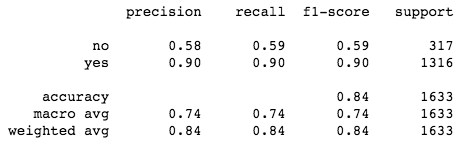
\includegraphics[scale=0.45]{latex/images/spatialscore.png}
\label{fig:HeatmapAfter}
\caption{Scores for spatial questions}
\end{figure}



\subsection{Discussion}

We should treat neural models as a theory or brain that is applicable and functional for every task scenario \cite{regier1996human}  



However, color questions could get more complex as "people employ compositional color descriptions to express meanings not covered by basic terms, such as greenish-blue" \cite{monroe2016learning}. It would be shallow to assume that color questions are simplistic, especially if we expect the system to answer colors beyond the basic color terms like "green" and "red." 

\cite{monroe2017colors}


intersective compostionality: intersective compositionality is when two words which one is attributed to the meaning of the other "brown bear" where it means a bear that is brown-[brown and bear] 

non-intersective compostionality: non-intersective is one word does not modify the second, such as [Teddy bear]. 'Teddy bear' cannot be mean a bear that is 'Teddy', 'Teddy' is not an attribute of a bear so not [Teddy + bear]. Teddy + bear is instead a different entity with a different perceptual meaning. 

\cite{larsson-2017-compositionality} 